\chapter{Swaths and turns}
\label{ch:swaths}

Once the headland is mowed (Chapter~\ref{ch:headlands}), the region left
inside it, the \emph{interior}, is mowed by parallel straight passes. This
chapter places these passes, studies the turn from the end of one to the
start of another, chooses the order in which they are driven and the
direction they run in, and puts everything together into a first complete
plan. It deals with interiors that every line in the direction of the
passes crosses at most once; Chapter~\ref{ch:split} cuts the other ones into
such pieces.

\section{The swaths}

\begin{definition}{Swath}{swath}
  For a direction $\theta$, with $u = (\cos\theta, \sin\theta)$ and $n =
  (-\sin\theta, \cos\theta)$, a \emph{swath} is the segment followed by the
  centre of the deck during a pass: a piece of a line $\{p : p \cdot n =
  q\}$ inside the interior, where $q$ is its \emph{lateral position}. The
  rear axle follows the same line, a distance $d$ behind the deck's centre.
\end{definition}

Let $q_0$ and $q_1$ be the smallest and the largest value of $p \cdot n$ over
the interior: $W = q_1 - q_0$ is its \emph{width} across the direction
$\theta$. The first pass must cut up to the edge of the interior, with the
same overlap $o$ as between two passes, so its deck's centre is at $q_0 +
w/2 - o$; likewise the last one is at $q_1 - w/2 + o$, and the passes in
between are $s = w - o$ apart.

\begin{proposition}{Number of passes}{passcount}
  An interior of width $W \ge w - 2o$ across $\theta$ needs
  \[
    N = 1 + \Bigl\lceil \frac{W - w + 2o}{s} \Bigr\rceil
  \]
  passes, at the lateral positions $q_0 + w/2 - o + i s$ for $i = 0, \dots,
  N - 2$, and $q_1 - w/2 + o$ for the last one.
\end{proposition}

\begin{proof}
  The first and the last positions are $(q_1 - w/2 + o) - (q_0 + w/2 - o) =
  W - w + 2o$ apart. With a spacing of at most $s$, at least $(W - w + 2o)/s$
  gaps are needed between them, so $\lceil (W - w + 2o)/s \rceil$ gaps and
  one more pass than gaps. Placing the passes $s$ apart from the first and
  moving the last one back onto $q_1 - w/2 + o$ makes the last gap at most
  $s$.
\end{proof}

\begin{example}{The interior of the rectangle}{rectinterior}
  With two headland passes the interior of the rectangle is
  \SI{16.06}{\metre} by \SI{8.06}{\metre}. With passes along the long side
  ($\theta = 0$), $W = 8.06$ and
  \[
    N = 1 + \Bigl\lceil \frac{8.06 - 0.97 + 2 \times 0.05}{0.92}
      \Bigr\rceil = 1 + \lceil 7.815 \rceil = 9 .
  \]
\end{example}

Along its length, a swath stops a distance $r$ (the radius of a blade)
before the edge of the interior: the front of the blades then reaches the
edge, which is what Proposition~\ref{prop:headlandcount} assumed when it
counted the headland passes.

\section{Where a pass ends and the next begins}
\label{sec:shift}

The deck is ahead of the rear axle. At the end of a pass the deck's centre
is on the line where the swaths stop, and the rear axle is $d$ behind it,
inside the interior. The next pass, driven the other way, starts with its
deck's centre on the same line, so its rear axle is $d$ behind that line,
outside the interior (Figure~\ref{fig:shift}).

\begin{inwords}
  Between the end of a pass and the start of the next, the rear axle must
  move a distance $2d$ further out, towards the border. Every turn at the
  end of a pass is a turn from the pose $(0, 0, 0)$ to the pose $(2d,
  \Delta, \pi)$, where $\Delta$ is the lateral distance to the next pass
  (with $d = \SI{0.55}{\metre}$, $2d = \SI{1.10}{\metre}$).
\end{inwords}

The turns of Chapter~\ref{ch:paths} went from $(0, 0, 0)$ to $(0, \Delta,
\pi)$. The shift makes the three-point turn to the next pass a little
slower ($\SI{10.69}{\second}$ against $\SI{10.65}{\second}$ in
Example~\ref{ex:threepoint}), and the mower reaches further: its outline
goes up to $a_{\mathrm{turn}} = \SI{2.62}{\metre}$ beyond the rear axle at
the end of the pass, the room that the headland must leave.

\begin{figure}[ht]
  \centering
  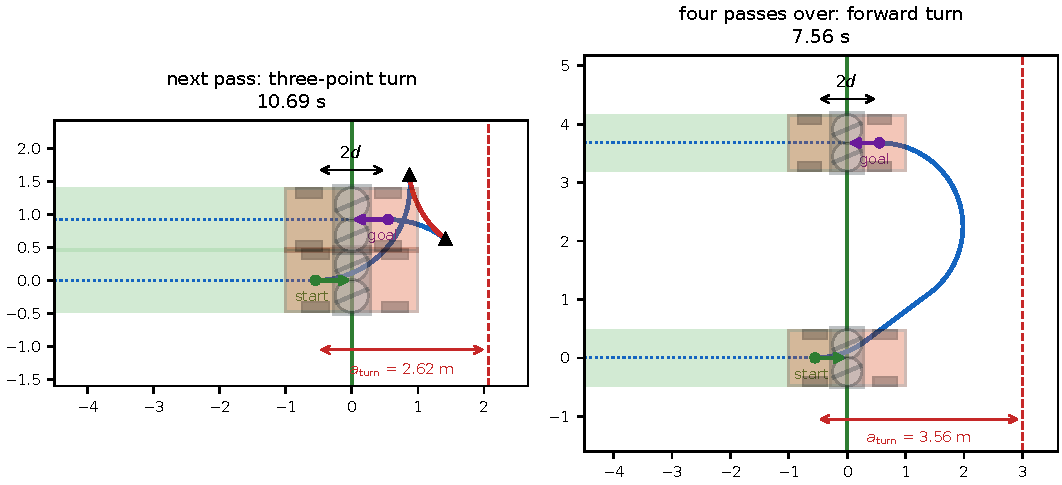
\includegraphics[width=\textwidth]{figures/shift}
  \caption{The end of a pass (start, green arrow: the rear axle) and the
    start of the next one driven the other way (goal, purple arrow), with
    the mower drawn at both poses: the decks are on the same line (green,
    the edge of the region to mow, where the swaths stop), so the rear axles
    are $2d$ apart. The path of the rear axle is blue forward and red
    reverse; black triangles mark the changes of direction. The red dashed
    line is the farthest point reached by the mower's outline. Left: to the
    next pass, $\Delta = \SI{0.92}{\metre}$, a three-point turn. Right: four
    passes over, $\Delta = \SI{3.68}{\metre}$, a forward turn, faster but
    reaching \SI{0.94}{\metre} further.}
  \label{fig:shift}
\end{figure}

\section{Turning over a jump}

Since $s = \SI{0.92}{\metre}$ is much less than $2\Rmin =
\SI{2.86}{\metre}$, the mower cannot turn forward into the next pass without
a loop (Section~\ref{sec:nextpass}). It can, however, turn forward into a
pass further away.

\begin{proposition}{Forward turn over a jump}{forwardturn}
  For $\Delta \ge 2R$, the path that turns left at radius $R$, goes straight,
  and turns left again at radius $R$ ($L^+S^+L^+$) from $(0, 0, 0)$ to $(2d,
  \Delta, \pi)$ has length
  \[
    \ell = \pi R + \sqrt{(2d)^2 + (\Delta - 2R)^2},
  \]
  of which $\pi R$ on arcs and the rest on the straight line.
\end{proposition}

\begin{proof}
  Turning left from $(0, 0, 0)$, the rear axle goes round the centre $c_1 =
  (0, R)$. Arriving at $(2d, \Delta)$ with heading $\pi$ while turning left,
  it goes round the centre $c_2 = (2d, \Delta) + R(0, -1) = (2d, \Delta -
  R)$, since the centre is on the left of the heading. A straight line
  touching two circles of the same radius, both driven counter-clockwise,
  is parallel to $c_2 - c_1 = (2d, \Delta - 2R)$ and as long as it: its
  length is $\sqrt{(2d)^2 + (\Delta - 2R)^2}$. Its heading $\beta =
  \operatorname{atan2}(\Delta - 2R, 2d)$ is in $[0, \pi/2)$ when $\Delta
  \ge 2R$. The first arc turns the heading from $0$ to $\beta$, the second
  from $\beta$ to $\pi$: together they turn by $\pi$ and their length is
  $\pi R$.
\end{proof}

When $\Delta < 2R$, the angle $\beta$ is negative and the first arc would
have to turn by $2\pi + \beta$, a loop. For $\Delta$ a little below $2R$ the
shortest forward path starts with a short right turn instead ($R^+S^+L^+$):
this is what happens three passes over, $\Delta = \SI{2.76}{\metre}$, where
it costs \SI{0.15}{\metre} of right turn.

\begin{example}{Four passes over}{fourover}
  With $R = \SI{1.430}{\metre}$, $2d = \SI{1.10}{\metre}$ and $\Delta = 4 s
  = \SI{3.68}{\metre}$:
  \[
    \ell = \pi \times 1.430 + \sqrt{1.10^2 + (3.68 - 2.860)^2}
         = 4.493 + 1.372 = \SI{5.865}{\metre}.
  \]
  At \SI{0.7}{\metre\per\second} on the arcs and \SI{1.2}{\metre\per\second}
  on the straight line, it takes
  \[
    t = \frac{4.493}{0.7} + \frac{1.372}{1.2} = 6.418 + 1.143
      = \SI{7.56}{\second},
  \]
  against \SI{10.69}{\second} for the three-point turn to the next pass.
\end{example}

Figure~\ref{fig:turntimes} shows the time of the fastest turn and the room
it needs for jumps of one to ten passes. The fastest turns over one and two
passes have reverse legs; from three passes on they are forward turns, which
are fastest at three or four passes over and then grow by about
\SI{0.7}{\second} per pass. The forward turns need more room:
$a_{\mathrm{turn}} = \SI{3.56}{\metre}$ instead of \SI{2.62}{\metre}.

\begin{figure}[ht]
  \centering
  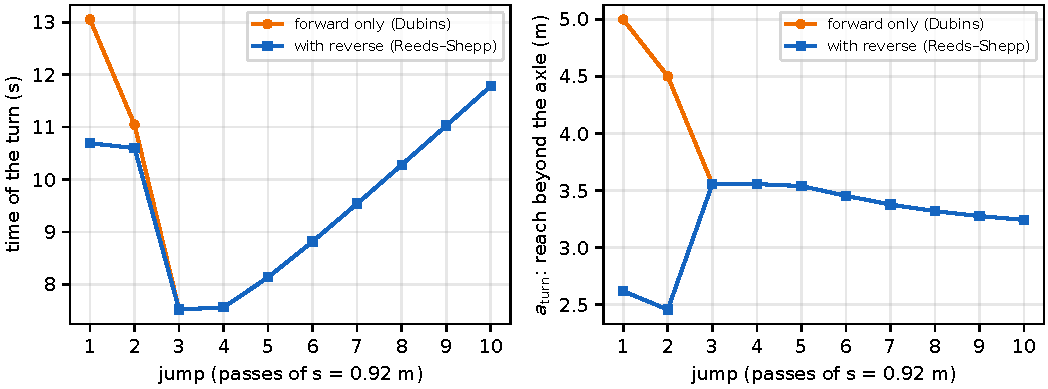
\includegraphics[width=\textwidth]{figures/turn_times}
  \caption{Turns from the end of a pass to a pass a number of passes away,
    driven the other way, with the shift $2d$ of Section~\ref{sec:shift}.
    Left: the time of the fastest turn, forward only (orange) and with
    reverse allowed (blue); the two are the same from three passes on.
    Right: how far the outline reaches beyond the rear axle at the end of
    the pass, which sets the depth of the headland.}
  \label{fig:turntimes}
\end{figure}

\section{The order of the passes}

Driving the passes in their lateral order, $0, 1, 2, \dots$, every turn is
a three-point turn. Any other order is allowed: as long as every pass is
driven the other way from the one before, the mower always turns at the
same end of the passes it joins. The order is then a sequence visiting
every pass once, and its cost is the sum of the times of its turns.

\begin{definition}{Pass order}{passorder}
  For $N$ passes and the turn time $T(j)$ over a jump of $j$ passes, a
  \emph{pass order} is a permutation $(\pi_1, \dots, \pi_N)$ of $\{0, \dots,
  N - 1\}$, and its cost is
  \[
    C(\pi) = \sum_{k=1}^{N-1} T\bigl(|\pi_{k+1} - \pi_k|\bigr).
  \]
\end{definition}

This is the problem of the shortest path through all the points of a
travelling salesman, on points that lie on a line but with an unusual
distance ($T$ is not increasing with the jump). It was posed for field
operations by Bochtis and Vougioukas~\cite{bochtis2008minimising}, who
report savings of up to half of the non-working distance. For a few dozen
passes a
local search finds very good orders. The code starts from the lateral order
and from interleaved blocks ($i, i + k, i + 1, i + k + 1, \dots$ for $k = 2,
\dots, 7$), and improves each of them while one of two moves lowers the
cost:

\begin{description}
  \item[Reversal (2-opt).]
    \leavevmode\\
    Drive a stretch of the sequence backwards:
    \[
      (\dots, \pi_i, \pi_{i+1}, \dots, \pi_j, \dots) \;\to\;
      (\dots, \pi_j, \dots, \pi_{i+1}, \pi_i, \dots).
    \]
  \item[Move (or-opt).]
    \leavevmode\\
    Take a run of one to three consecutive passes out of the sequence and
    put it back elsewhere, in either direction.
\end{description}

\begin{example}{Nine passes}{ninepasses}
  With $T(1) = 10.69$, $T(2) = 10.60$, $T(3) = 7.52$, $T(4) = 7.56$, $T(5)
  = \SI{8.13}{\second}$, the lateral order of nine passes costs $8 \times
  10.69 = \SI{85.5}{\second}$. The local search finds the order
  \[
    8, 5, 1, 4, 7, 2, 6, 3, 0,
  \]
  with jumps $3, 4, 3, 3, 5, 4, 3, 3$: all forward turns, for
  \[
    C = 5 \times 7.52 + 2 \times 7.56 + 8.13 = \SI{60.85}{\second}.
  \]
\end{example}

The gain has a price: the headland must leave room for the forward turns.
With $a_{\mathrm{turn}} = 3.556$ in Proposition~\ref{prop:headlandcount},
\[
  n = 1 + \Bigl\lceil \frac{3.556 + 0.05 - 0.80 - 0.615 - 0.485}{0.92}
    \Bigr\rceil = 1 + \lceil 1.854 \rceil = 3
\]
headland passes instead of two. The third ring cuts a band that passes
would have cut otherwise, so the total length mowed hardly changes, but the
ring has corners, and there are fewer, longer passes to turn between.
Whether the order with jumps pays off depends on the lawn: the planner
computes both (the patterns \code{adjacent} and \code{skip}) and the
results below compare them.

\section{The direction of the passes}

The time to mow the interior is roughly the length of the passes at mowing
speed plus one turn per pass. The total length of the passes is close to
the area of the interior divided by $s$, whatever the direction, while the
number of turns follows the width $W(\theta)$ through
Proposition~\ref{prop:passcount}. The direction that makes the interior
narrowest is therefore a good choice.

\begin{theorem}{Minimum width}{minwidth}
  The width $W(\theta)$ of a polygon, over all directions $\theta$, is
  smallest when $\theta$ is the direction of an edge of its convex hull.
\end{theorem}

\begin{proof}
  The width only depends on the extreme values of $p \cdot n(\theta)$, which
  are reached at vertices of the convex hull; take its vertices $v_i$. Over
  an interval of directions where the same vertex $v_a$ gives the largest
  value and the same vertex $v_b$ the smallest,
  \[
    W(\theta) = (v_a - v_b) \cdot n(\theta) = |v_a - v_b| \cos(\theta -
    \gamma)
  \]
  for a fixed angle $\gamma$. This is positive on the interval, so $\theta -
  \gamma$ stays in $(-\pi/2, \pi/2)$, where the cosine is concave: $W$ is
  concave on the interval and its smallest value there is at one of its
  ends. The ends are the directions where $v_a$ or $v_b$ changes, that is,
  where $n(\theta)$ is perpendicular to an edge of the hull: $\theta$ is
  then the direction of that edge.
\end{proof}

Houle and Toussaint~\cite{houle1988computing} use this property to compute
the width of a set of points; for a convex polygon, the computation takes
time linear in its number of vertices.

The planner estimates the time for the directions of the edges of the
convex hull, and for every multiple of $15°$ (the ceiling in the number of
passes and the lengths of the passes make the estimate differ a little from
the width), and keeps the fastest. Figure~\ref{fig:direction} shows the
estimate for the interiors of the rectangle and the L-shape: the passes run
along the long side, in both cases at $\theta = 0$.

\begin{figure}[ht]
  \centering
  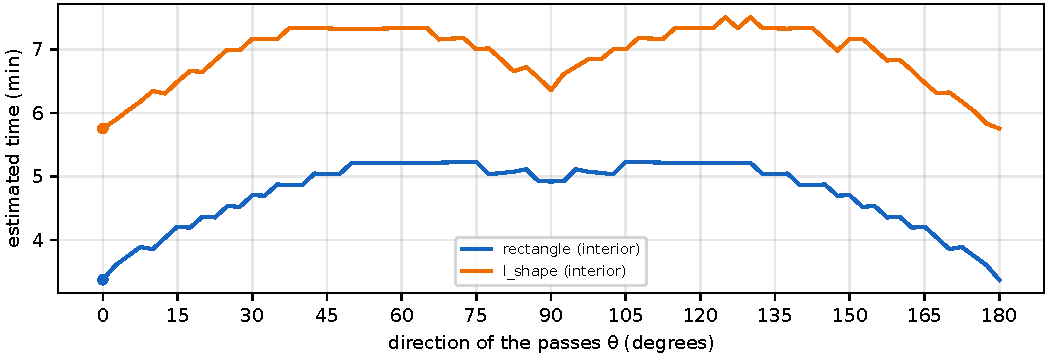
\includegraphics[width=\textwidth]{figures/direction}
  \caption{Estimated time to mow the interior left by two headland passes,
    against the direction of the passes: the length of the passes at
    \SI{1.2}{\metre\per\second}, plus \SI{10.69}{\second} per turn. The dots
    are the minima, at $\theta = 0$ (passes along the $x$ axis) for both
    lawns. The steps come from the number of passes, a whole number.}
  \label{fig:direction}
\end{figure}

\section{When a turn does not fit}

On a straight border perpendicular to the passes, the headland leaves the
room $a_{\mathrm{turn}}$. On an oblique border, the end of the next pass is
further along it, and near the corners of the interior the border may be
closer than expected. For each turn, the planner tries the Reeds--Shepp
paths from the end of the pass to the start of the next, fastest first,
and keeps the first one that the collision checker of
Chapter~\ref{ch:headlands} accepts. If none fits, it stops the previous
pass a distance $c_p$ early and starts the next one a distance $c_n$ late,
for the pairs $(c_p, c_n)$ on a grid of \SI{0.25}{\metre} up to
\SI{3}{\metre}, in increasing order of $c_p + c_n$; the blades stay
engaged during the turn, which cuts most of what the shortened passes
leave. If still nothing fits, it searches a path around the obstacle (the
search of Chapter~\ref{ch:order}).

The first pass is reached from the end of the headland with the blades off.
The order may be driven forwards or backwards, and the first pass in
either direction; of these four starts the planner keeps the one with the
fastest connection.

\section{A complete plan}

Headland and passes together make a complete plan. Figure~\ref{fig:patterns}
and the table below show it on the rectangle with both orders, and on the
L-shape with the lateral order.

\begin{figure}[p]
  \centering
  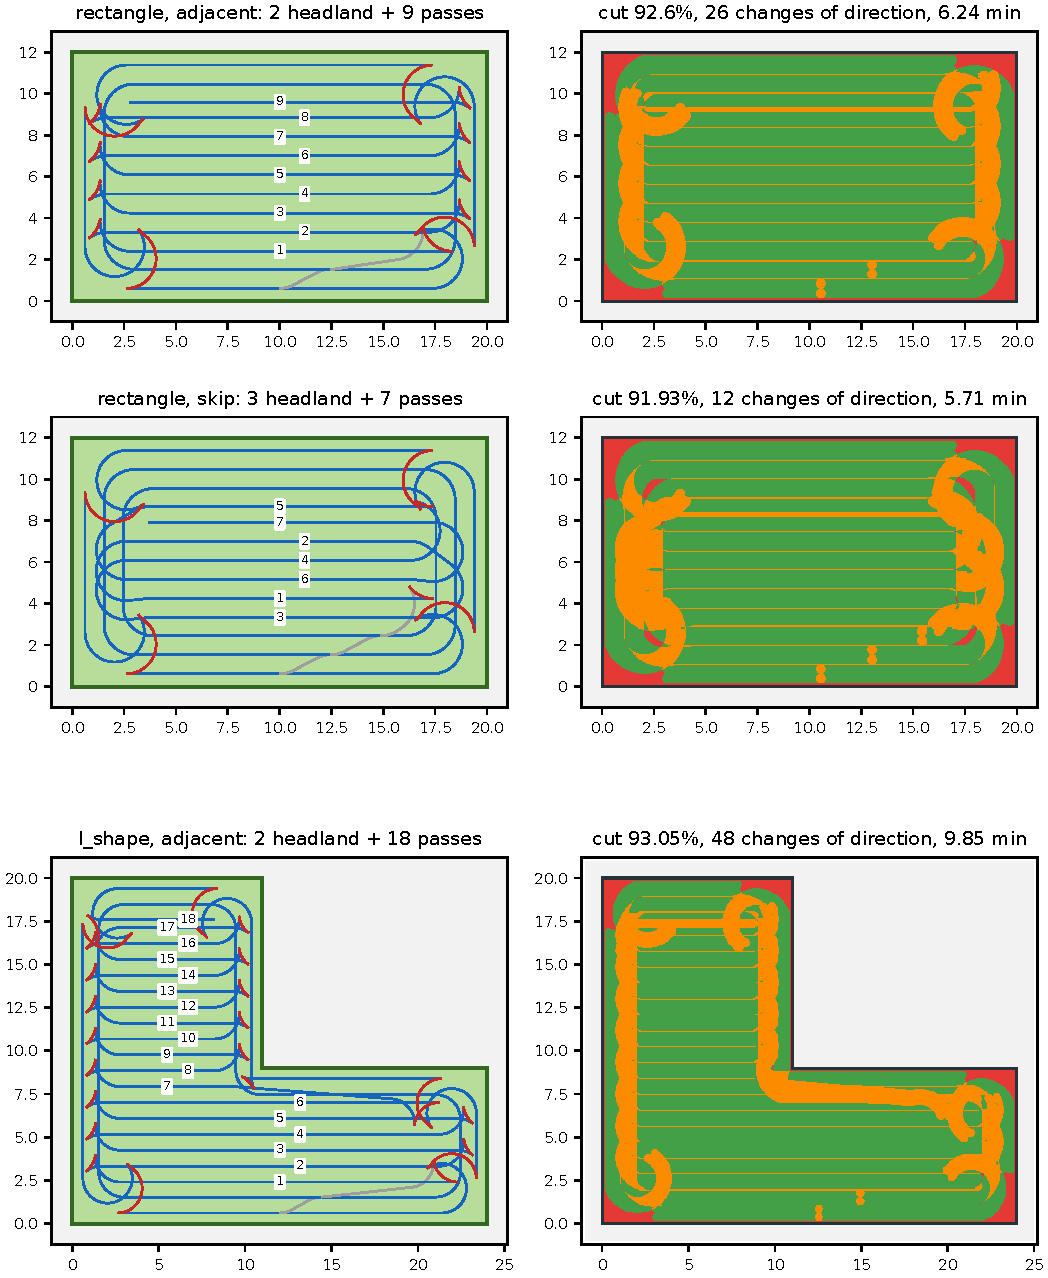
\includegraphics[width=\textwidth]{figures/patterns}
  \caption{Complete plans: headland passes, then the interior (numbers: the
    order of the passes). Top: the rectangle with the lateral order, two
    headland passes and nine three-point turns. Middle: the order with
    jumps, three headland passes and only forward turns. Bottom: the
    L-shape with the lateral order; between the 6th and the 7th pass the
    mower crosses from one arm to the other, mowing what it has already
    mowed.}
  \label{fig:patterns}
\end{figure}

\begin{center}
\begin{tabular}{@{}llrrrrr@{}}
  \toprule
  lawn & order & headland & passes & cut & changes & time \\
  \midrule
  rectangle & adjacent & 2 & 9 & 92.6\% & 26 & \SI{6.24}{\minute} \\
  rectangle & skip & 3 & 7 & 91.9\% & 12 & \SI{5.71}{\minute} \\
  L-shape & adjacent & 2 & 18 & 93.1\% & 48 & \SI{9.85}{\minute} \\
  L-shape & skip & 3 & 16 & 92.6\% & 20 & \SI{9.95}{\minute} \\
  \bottomrule
\end{tabular}
\end{center}

On the rectangle the order with jumps saves half a minute, 8.5\%, with half
as many changes of direction. On the L-shape it does not: the cost $T(j)$
assumes that every pass ends on the same line, but here the passes of the
two arms end in different places, and the jumps send the mower from one
arm to the other. The uncut \SI{7}{\percent} or so is the strip along the
border and the corners of the lawn left by the headland
(Chapter~\ref{ch:headlands}), plus small gaps where the rings meet the
passes.

\begin{inwords}
  Parallel passes cost one turn each, so they run across the smallest width
  of the interior. A car-like mower cannot turn forward into the next pass,
  only into a pass three or more widths away; driving the passes in an order
  that jumps over a few of them turns three-point turns into forward turns,
  at the cost of a wider headland. Both choices assume that the passes are
  regular; lawns whose passes are not, like the L-shape, are cut into
  regular pieces in the next chapter.
\end{inwords}

\begin{incode}
  \code{mowersim/planning/swaths.py}: \code{swaths}
  (Definition~\ref{def:swath}, Proposition~\ref{prop:passcount}),
  \code{turn\_time} and \code{turn\_ahead} (the turn from $(0, 0, 0)$ to
  $(2d, \Delta, \pi)$), \code{min\_forward\_jump}, \code{pass\_order},
  \code{improve\_order} (2-opt and or-opt), \code{candidate\_directions}
  and \code{best\_direction} (Theorem~\ref{thm:minwidth}), \code{join}
  (shortening the passes until the turn fits), \code{plan\_passes} and
  \code{plan\_simple}, the complete planner of this chapter:
  \begin{verbatim}
python -m mowersim plan lawns/rectangle.json --pattern skip
  \end{verbatim}
\end{incode}
